
\section{Auswertung}

Die verwendete Schaltung hatte die folgenden Daten.

\begin{align*}
  L &= \SI{3,53(3)}{\milli\henry} \\
  C &= \SI{5,015(15)}{\nano\farad} \\
  R_1 &= \SI{30,3(1)}{\ohm} \\
  R_2 &= \SI{271,6(3)}{\ohm}
\end{align*}

\subsection{Einhüllende der Schwingungskurve}

Die Wertepaare ($U_C(t_i), t_i$) müssen für die Ausgleichsrechnung an die Funktion
\eqref{eqn:exp} bestimmt werden.
Die Werte $U_C(t_i)$ wurden mit dem Cursor des Oszilloskops gemessen.
Hingegen wurden die Zeiten $t_i$ aus dem Bild der Schwingungskurve mit
Hilfe eines Lineals abgelesen. Ein Abbild der Schwingungskurve ist in Abb.
\ref{fig:Schwingungskurve} dargestellt.

\begin{figure}
  \centering
  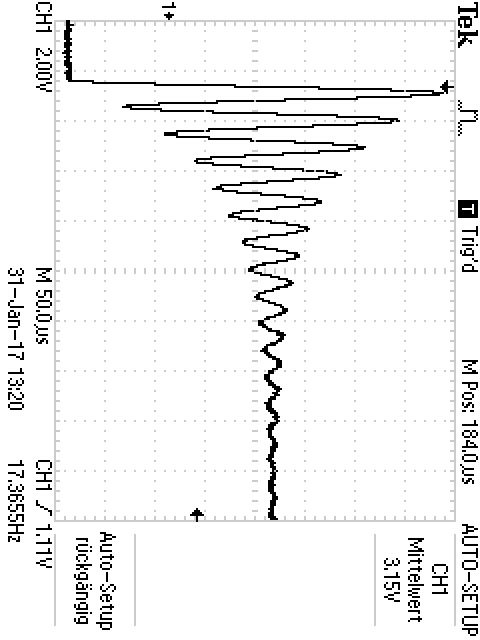
\includegraphics[width=\textwidth, angle=90, height=8cm]{F0001TEK.JPG}
  \caption{Gemessene Spannungsamplituden in Abhängigkeit der Zeit bei der Messung
  der gedämpften Schwingung in dem ersten Teil der Messung.}
  \label{fig:Schwingungskurve}
\end{figure}

Die Schwingungskurve in Abb. \ref{fig:Schwingungskurve} wurde beim
Widerstand $R_1$ und einer Generatorfrequenz von $\SI{5,82}{\hertz}$ erstellt.

Die diskreten Wertepaare ($U_C(t_i), t_i$) sind in der Tabelle \ref{tab:Schwingungskurve}
dargestellt. Dabei wurden für $U_C(t_i)$ jeweils die Maxima der Schwingungskurve
vermessen.

In der Abb. \ref{fig:Schwingungskurve} ist die Referenzlinie bezüglich der die Maxima
vermessen sind, die niederigste Linie an der linken Seite.

\floatplacement{table}{htbp}
\begin{table}
 \centering
 \sisetup{table-format=3.2}
 \begin{tabular}[width=\textwidth]{S S}
     \toprule
      {Zeit in $\si{\micro\second}$} & {Maxima in $\si{\volt}$} \\
     \midrule
      0,0 & 15,08 \\
      27,5 & 13,20 \\
      55,0 & 11,92 \\
      82,5 & 10,96 \\
      112,5 & 10,24 \\
      142,5 & 9,68 \\
      172,5 & 9,36 \\
      202,5 & 9,04 \\
      235,0 & 8,88 \\
      267,5 & 8,76 \\
      302,5 & 8,64 \\
      337,5 & 8,52 \\
      \bottomrule
  \end{tabular}
  \caption{Messdaten der Schwingungskurve.}
  \label{tab:Schwingungskurve}
\end{table}

Mit den Wertepaaren aus Tabelle \ref{tab:Schwingungskurve} wurde mittels
des \emph{Python}-Paketes \emph{curve\_fit} eine Ausgleichsrechnung an eine
exponentielle Funktion der Form

\begin{align}
  \label{eqn:exp}
  U\ua{c}(t) = a\cdot\exp^{-b\cdot t} + c
\end{align}

durchgeführt. Für die Parameter ergeben sich somit die Werte

\begin{align*}
  a & = \SI{6,62(3)}{\volt} \\
  b &= \num{1,17(1)e4}\frac{1}{\si{\second}} \\
  c &= \SI{8,44(2)}{\volt}
\end{align*}

Die Ausgleichfunktion ist mit den Daten aus Tabelle \ref{tab:Schwingungskurve} in Abb. \ref{fig:Ausgleichsrechnung} dargestellt.

\floatplacement{table}{htbp}
\begin{figure}
  \centering
  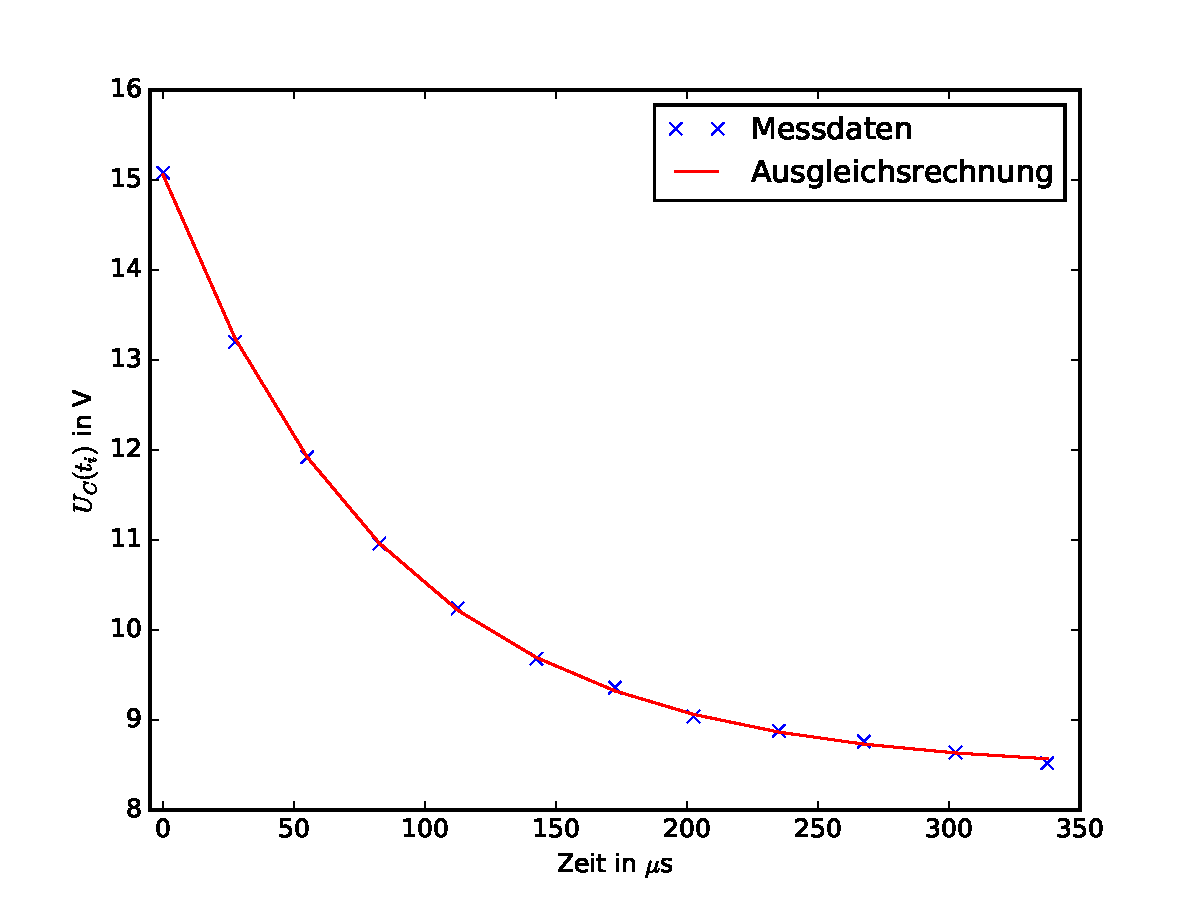
\includegraphics[width=\textwidth]{ausgleichsrechnung.pdf}
  \caption{Darstellung der Ausgleichsfunktion.}
  \label{fig:Ausgleichsrechnung}
\end{figure}

Der Exponent der Ausgleichsfunktion $b$ liefert über die Formeln
\eqref{eqn:R_eff} und \eqref{eqn:T_ex}
den effektiv Widerstand $R\ua{eff}$ und die Abklingzeit $T\ua{ex}$.

\begin{equation}
  \label{eqn:R_eff}
  R\ua{eff} = 2 b L
\end{equation}

\newpage

Damit ergeben sich die folgenden Werte.

\begin{align*}
  R\ua{eff} &= \SI{82,4(12)}{\ohm}\\
  T\ua{ex} &= \SI{8,56(1)e-5}{\second}
\end{align*}

Im Vergleich zu dem eigebauten, verwendeten Widerstand $R_1$ fällt auf, dass
$R\ua{eff}$ deutlich größer ist. Dies ist damit zu begründen, dass $R\ua{eff}$
den Innenwiderstand des Generators mit einbezieht, welcher in $R_1$ nicht erfasst
wird.

\subsection{Widerstand im aperiodischen Grenzfall}

Aus den Daten $L$ und $C$ der Apparatur lässt sich über den Zusammenhang:

\begin{equation*}
  R\ua{ap} = 2\cdot \sqrt{\frac{L}{C}}
\end{equation*}

der Widerstand des aperiodischen Grenzfalles $R\ua{ap}$ errechnen.
Der Wert $R\ua{ap}$ wurde auch experimentell bestimmt. Die Messung ergeben
die folgenden Werte.

\begin{align*}
  R\ua{ap,theo} &= \SI{1678(8)}{\ohm}\\
  R\ua{ap} &= \SI{2700}{\ohm}
\end{align*}

Die Messung wurde bei einer Frequenz von $\nu = \SI{5,82}{\hertz}$ erhoben.
Der Wert $R\ua{ap}$ ist der experimentell bestimmte Wert. Dieser wurde an
dem variablen Widerstand der Apparatur abgelesen und wird als fehlerfrei
angenommen.

\subsection{Resonanzfrequenz}

Die Resonanzfrequenz lässt sich mit den Apparaturdaten über die Formel \eqref{eqn:omega_res}
errechnen. Aus der Kreisfreqeunz lässt sich durch Multiplikation mit
$2\pi$ direkt die Frequenz $nu\ua{res}$ errechnen.
Als Widerstand wurde der gemessene effektiv Widerstand $R\ua{eff}$
verwendet.
Die berechnete Resonanzfrequenz beträgt:

\begin{align*}
  \nu\ua{res} &= \SI{3.774(17)e4}{\hertz}.
\end{align*}

\newpage

In dem Diagramm \ref{fig:Kondensator_Frequ} ist die normierte Kondensatorspannung
in Abhängigkeit von der Frequenz dargestellt. Mit normiert ist gemeint, dass die
Kondensatorspannung durch die Generatorspannung geteilt wird.
Das Diagramm \ref{fig:Kondensator_Frequ} wurde mit den Daten aus Tabelle \ref{tab:Kondensator_Frequ}
erstellt.

\floatplacement{table}{htbp}
\begin{figure}
  \centering
  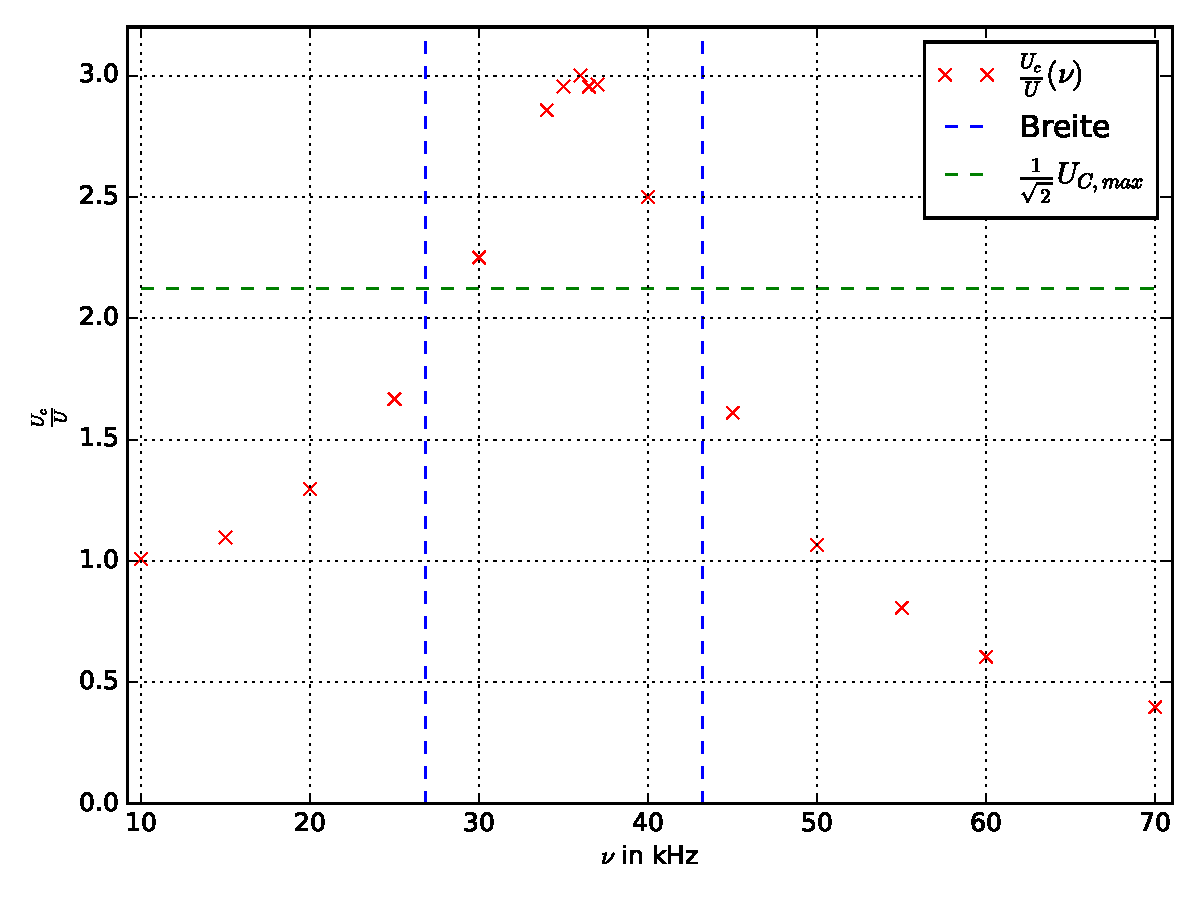
\includegraphics[width=\textwidth]{messung_c.pdf}
  \caption{Normierte Kondensatorspannung in Abhängigkeit von der Frequenz.}
  \label{fig:Kondensator_Frequ}
\end{figure}

Der Maximalwert der Kondensatorspannung wird bei einer Frequenz von

\begin{equation}
  \label{eqn:Resonanzfrequenz}
  \nu\ua{res,1} = \SI{36}{\kilo\hertz}
\end{equation}

gemessen. Die Halbwertsbreite der Kondensatorspannung ist durch die Differenz der Werte
$\nu_+$ und $\nu_-$ gegeben.

\begin{align*}
  \nu_+ &\approx \SI{27}{\kilo\hertz} \\
  \nu_- &\approx \SI{43}{\kilo\hertz}
\end{align*}

Damit ergibt sich die Breite zu $\approx \SI{16}{\kilo\hertz}$.

Der dazugehörigen Theoriewerte kann durch die Formel \eqref{eqn:breite} berechnet
werden und ist im folgenden angegeben:

\begin{equation}
  \label{eqn:breite}
  \text{Breite} \approx \frac{R\ua{eff}}{L}
\end{equation}

\begin{align*}
  \text{Breite}\ua{theo} &= \SI{27,53(27)}{\kilo\hertz} .\\
\end{align*}

Die Werte weichen nur geringfügig voneinander ab.
Die Güte $q$ des Schwingkreises ist der Maximalwert des Verhältnises von
Kondensatorspannung zur Generatorspannung.
In Abb. \ref{fig:Kondensator_Frequ} ist das Maximalverhältnis bei der
Resonanzfrequenz erreicht. An diesem Punkt beträgt das Verhältnis

\begin{equation*}
  q = 3.
\end{equation*}

Der errechnete Wert liegt bei $q\ua{theo} = \num{3,24(4)}$.

\subsubsection{Resonanzfrequenz aus der Phasenverschiebung}

Aus der Phasenverschiebung zwischen Generator- und Kondensatorspannung in Abhängigkeit
von der Frequenz kann die Resonanzfrequenz $\nu\ua{res}$ bestimmt werden.
Die Resonanzfrequenz ist der Wert, an dem die Phase zwischen den Spannungen
$\varphi\ua{res} = \frac{\pi}{2}$ entspricht.
Der gemessene Wert wurde aus dem Diagramm \ref{fig:Resonanz} abgelesen.

Die Daten der Messung zur Resonanzfrequenz sind in der Tabelle \eqref{tab:Kondensator_Frequ} dargestellt.

\floatplacement{table}{htbp}
\begin{table}
 \centering
 \sisetup{table-format=2.1}
 \begin{tabular}[width=\textwidth]{S S S S S}
     \toprule
      {$\nu_G$ in $\si{\kilo\hertz}$} & {$\lambda$ in $\si{\micro\second}$} & {$\varphi$ in $\si{\micro\second}$} & {$U\ua{G}$ in $\si{\volt}$} & {$U\ua{C}$ in $\si{\volt}$} \\
     \midrule
      10 & 98,0 &   0    &  5,4  & 5,4 \\
      15 & 67,0 &   1,2  &  5,4  & 5,9 \\
      20 & 50,8 &   1,6  &  5,1  & 6,6 \\
      25 & 40,0 &   2,0  &  5,0  & 8,4 \\
      30 & 33,2 &   3,2  &  4,8  & 10,8 \\
      34 & 29,6 &   4,8  &  4,5  & 12,8 \\
      35 & 28,4 &   5,2  &  4,4  & 13,0 \\
      36 & 28,0 &   6,4  &  4,4  & 13,2 \\
      36,5 & 27,2 & 6,0  &  4,4  & 13,0 \\
      37 & 26,4 &   6,8  &  4,3  & 12,8 \\
      40 & 25,2 &   7,8  &  4,5  & 11,2 \\
      45 & 22,2 &   8,4  &  4,7  & 7,6 \\
      50 & 19,8 &   8,6  &  4,9  & 5,2 \\
      55 & 18,2 &   8,2  &  5,0  & 4,0 \\
      60 & 16,6 &   8.0  &  5,0  & 3,0 \\
      70 & 14,0 &   7.0  &  5,0  & 2,0 \\
      \bottomrule
  \end{tabular}
  \caption{Messdaten zur Resonanzfrequenz.}
  \label{tab:Kondensator_Frequ}
\end{table}

\floatplacement{table}{htbp}
\begin{figure}
  \centering
  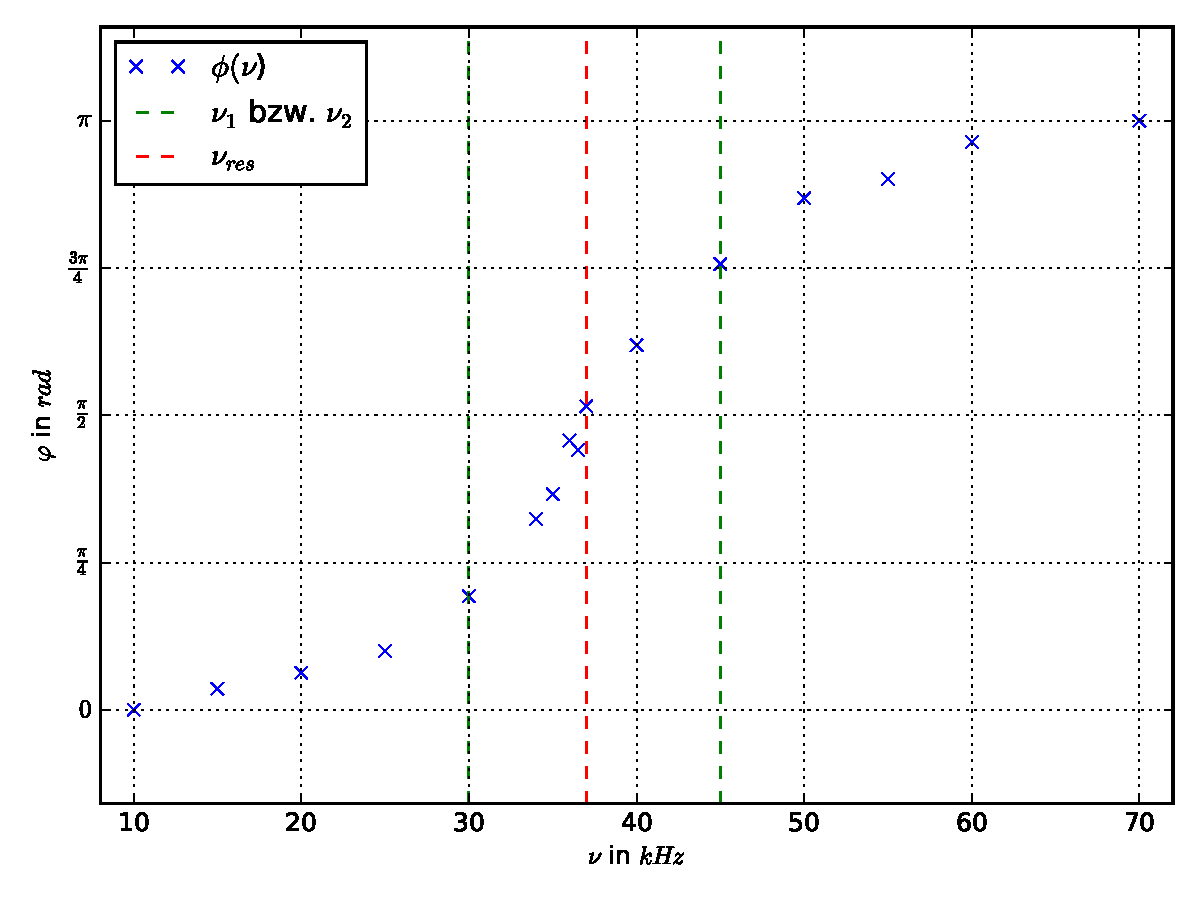
\includegraphics[width=\textwidth]{phase_gegen_nu.pdf}
  \caption{Phase zwischen Kondensator- und Generatorspannung in Abhängigkeit von der Frequenz.}
  \label{fig:Resonanz}
\end{figure}


Das Diagramm \ref{fig:Resonanz} wurde mit Daten aus der Tabelle
\ref{tab:Kondensator_Frequ} erstellt.
Der abgelesene Wert bei einer Phase von $\varphi\ua{res}$ ist:

\begin{equation*}
  \nu\ua{res,2} = \SI{37}{\kilo\hertz}.
\end{equation*}

Dieser Wert stimmt mit dem berechneten und in \eqref{eqn:Resonanzfrequenz} bestimmten
Wert nahezu überein.

Die Frequenz $\nu_1$, bei der die Freqeunz gerade $\frac{\pi}{4}$ ist, sowie die
Frequenz $\nu_2$, bei der $\varphi = \frac{3\pi}{4}$ ist sind dem Diagramm \ref{fig:Resonanz}
näherungsweise zu entnehmen.

\begin{align*}
  \nu_1 &\approx \SI{30}{\kilo\hertz} \\
  \nu_2 &\approx \SI{45}{\kilo\hertz}
\end{align*}

Rechnerisch ergeben sich $\nu_1$ und $\nu_2$ über den folgenden Zusammenhang.

\begin{align}
  \nu_1 &= (\frac{R}{2L} + \sqrt{\frac{R^2}{4L^2} + \frac{1}{LC}})\cdot \frac{1}{2\pi} \\
  \nu_2 &= (-\frac{R}{2L} + \sqrt{\frac{R^2}{4L^2} + \frac{1}{LC}})\cdot \frac{1}{2\pi}
\end{align}

$\nu_1$ und $\nu_2$ ergeben sich zu:

\begin{align*}
  \nu\ua{1,theo} &= \SI{36,21(17)}{\kilo\hertz} \\
  \nu\ua{2,theo} &= \SI{38,55(17)}{\kilo\hertz}
\end{align*}

Die Werte weichen deutlich von den gemessenen Werten ab.
Dies ist damit zu begründen, dass die gemessenen Werte nur Näherungen entsprechen.
Damit eine höhere Sicherheit der Messdaten besteht, hätten mehr Messwerte um den
Bereich einer Phasenverschiebung von $\varphi = \frac{\pi}{4}$ bzw.
$\varphi = \frac{3\pi}{4}$ genommen werden müssen. Es lässt sich aufgrund der
mangelnden Anzahl an Messwerten keine präzise Begründung für die signifikanten Unterschiede
zwischen den Theoriewerten und den gemessenen Werten machen.

\section{Diskussion}

Der effektiv Widerstand $R\ua{eff}$ weicht von dem angelegtem Widerstand $R\ua{1}$
ab, weil bei $R\ua{1}$ der Innenwiderstand des Generators, sowie der
Widerstand der verwendeten Kabel vernachlässigt worden ist.

Der gemessene Wert des Widerstandes im aperiodischen Grenzfall $R\ua{ap}$
weicht um ca. $\SI{900}{\ohm}$ von dem theoretisch berechneten Wert ab.
Der Innenwiderstand ist bei dem theoretischem Wert vernachlässigt
worden, weshalb der berechnete Widerstand niedriger sein muss als der gemessene.
Zudem hängt die Diskrepanz damit zusammen, dass der experimentelle Wert an der Apparatur
nur ungenau abgelesen werden konnte und vermutlich fehlerhaft ist. Es war somit nicht
sichergestellt, dass der abgelesene Widerstand tatsächlich mit dem angelegten
Widerstand übereinstimmt.

Darüberhinaus weichen die bestimmten Frequenzen $\nu_1$ und $\nu_2$ deutlich von den
berechneten Werten ab. Dies ist mit der geringfügigen Aussagekraft der wenigen
Messdaten in den Bereich von $\varphi = \frac{\pi}{4}$ und $\varphi = \frac{3\pi}{4}$
begründet. Im dem für $\nu_1$ und $\nu_2$ relevanten Messbereich wurde
jeweils lediglich ein Messwert erhoben. Es ist also verständlich, dass dieser
nicht mit dem berechnetem Wert übereinstimmt.

Die Güte der Apparatur weicht weicht um ca. $8\%$ von dem berechnetem Wert ab.
Dies ist im Rahmen der Messung als nicht signifikanter Unterschied zu betrachten.


\floatplacement{table}{htbp}
\begin{table}
 \centering
 \begin{tabular}[width=\textwidth]{S S}
     \toprule
     {Messgrößen} & {Messdaten} \\
     \midrule
      \text{Fitparameter} a & $\SI{6,62(3)}{\volt}$ \\
      \text{Fitparameter} b & $\SI{1,17(1)e4}{\per\second}$ \\
      \text{Fitparameter} c & $\SI{8,44(2)}{\volt}$ \\
      $R\ua{eff}$ & $\SI{82,4(12)}{\ohm}$ \\
      $T\ua{ex}$ & $\SI{8,56(1)e-5}{\second}$ \\
      $R\ua{ap}$ & $\SI{2700}{\ohm}$ \\
      $\nu\ua{res,1}$ & $\SI{36}{\kilo\hertz}$ \\
      $\nu\ua{+}$ & $\SI{27}{\kilo\hertz}$ \\
      $\nu\ua{-}$ & $\SI{43}{\kilo\hertz}$ \\
      q & 3 \\
      $\nu\ua{res,2}$ & $\SI{36}{\kilo\hertz}$ \\
      $\nu\ua{1}$ & $\SI{30}{\kilo\hertz}$ \\
      $\nu\ua{2}$ & $\SI{45}{\kilo\hertz}$ \\
      \bottomrule
  \end{tabular}
  \caption{Tabelle aller ermittelten Messgrößen.}
  \label{tab:Messdaten}
\end{table}
